% Created by tikzDevice version 0.10.1 on 2018-01-12 16:15:03
% !TEX encoding = UTF-8 Unicode
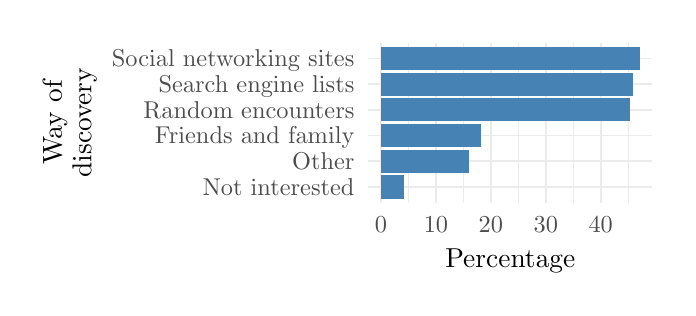
\begin{tikzpicture}[x=1pt,y=1pt]
\definecolor{fillColor}{RGB}{255,255,255}
\path[use as bounding box,fill=fillColor,fill opacity=0.00] (0,0) rectangle (231.26, 93.95);
\begin{scope}
\path[clip] (123.02, 30.77) rectangle (225.76, 88.45);
\definecolor{drawColor}{gray}{0.92}

\path[draw=drawColor,line width= 0.3pt,line join=round] (137.61, 30.77) --
	(137.61, 88.45);

\path[draw=drawColor,line width= 0.3pt,line join=round] (157.46, 30.77) --
	(157.46, 88.45);

\path[draw=drawColor,line width= 0.3pt,line join=round] (177.31, 30.77) --
	(177.31, 88.45);

\path[draw=drawColor,line width= 0.3pt,line join=round] (197.16, 30.77) --
	(197.16, 88.45);

\path[draw=drawColor,line width= 0.3pt,line join=round] (217.00, 30.77) --
	(217.00, 88.45);

\path[draw=drawColor,line width= 0.6pt,line join=round] (123.02, 36.35) --
	(225.76, 36.35);

\path[draw=drawColor,line width= 0.6pt,line join=round] (123.02, 45.66) --
	(225.76, 45.66);

\path[draw=drawColor,line width= 0.6pt,line join=round] (123.02, 54.96) --
	(225.76, 54.96);

\path[draw=drawColor,line width= 0.6pt,line join=round] (123.02, 64.26) --
	(225.76, 64.26);

\path[draw=drawColor,line width= 0.6pt,line join=round] (123.02, 73.57) --
	(225.76, 73.57);

\path[draw=drawColor,line width= 0.6pt,line join=round] (123.02, 82.87) --
	(225.76, 82.87);

\path[draw=drawColor,line width= 0.6pt,line join=round] (127.69, 30.77) --
	(127.69, 88.45);

\path[draw=drawColor,line width= 0.6pt,line join=round] (147.54, 30.77) --
	(147.54, 88.45);

\path[draw=drawColor,line width= 0.6pt,line join=round] (167.38, 30.77) --
	(167.38, 88.45);

\path[draw=drawColor,line width= 0.6pt,line join=round] (187.23, 30.77) --
	(187.23, 88.45);

\path[draw=drawColor,line width= 0.6pt,line join=round] (207.08, 30.77) --
	(207.08, 88.45);
\definecolor{fillColor}{RGB}{70,130,180}

\path[fill=fillColor] (127.69, 32.17) rectangle (135.96, 40.54);

\path[fill=fillColor] (127.69, 41.47) rectangle (159.33, 49.84);

\path[fill=fillColor] (127.69, 50.77) rectangle (163.85, 59.15);

\path[fill=fillColor] (127.69, 60.08) rectangle (217.70, 68.45);

\path[fill=fillColor] (127.69, 69.38) rectangle (218.83, 77.75);

\path[fill=fillColor] (127.69, 78.68) rectangle (221.09, 87.06);
\end{scope}
\begin{scope}
\path[clip] (  0.00,  0.00) rectangle (231.26, 93.95);
\definecolor{drawColor}{gray}{0.30}

\node[text=drawColor,anchor=base east,inner sep=0pt, outer sep=0pt, scale=  0.88] at (118.07, 33.32) {Not interested};

\node[text=drawColor,anchor=base east,inner sep=0pt, outer sep=0pt, scale=  0.88] at (118.07, 42.63) {Other};

\node[text=drawColor,anchor=base east,inner sep=0pt, outer sep=0pt, scale=  0.88] at (118.07, 51.93) {Friends and family};

\node[text=drawColor,anchor=base east,inner sep=0pt, outer sep=0pt, scale=  0.88] at (118.07, 61.23) {Random encounters};

\node[text=drawColor,anchor=base east,inner sep=0pt, outer sep=0pt, scale=  0.88] at (118.07, 70.54) {Search engine lists};

\node[text=drawColor,anchor=base east,inner sep=0pt, outer sep=0pt, scale=  0.88] at (118.07, 79.84) {Social networking sites};
\end{scope}
\begin{scope}
\path[clip] (  0.00,  0.00) rectangle (231.26, 93.95);
\definecolor{drawColor}{gray}{0.30}

\node[text=drawColor,anchor=base,inner sep=0pt, outer sep=0pt, scale=  0.88] at (127.69, 19.76) {0};

\node[text=drawColor,anchor=base,inner sep=0pt, outer sep=0pt, scale=  0.88] at (147.54, 19.76) {10};

\node[text=drawColor,anchor=base,inner sep=0pt, outer sep=0pt, scale=  0.88] at (167.38, 19.76) {20};

\node[text=drawColor,anchor=base,inner sep=0pt, outer sep=0pt, scale=  0.88] at (187.23, 19.76) {30};

\node[text=drawColor,anchor=base,inner sep=0pt, outer sep=0pt, scale=  0.88] at (207.08, 19.76) {40};
\end{scope}
\begin{scope}
\path[clip] (  0.00,  0.00) rectangle (231.26, 93.95);
\definecolor{drawColor}{RGB}{0,0,0}

\node[text=drawColor,anchor=base,inner sep=0pt, outer sep=0pt, scale=  0.99] at (174.39,  7.44) {Percentage};
\end{scope}
\begin{scope}
\path[clip] (  0.00,  0.00) rectangle (231.26, 93.95);
\definecolor{drawColor}{RGB}{0,0,0}

\node[text=drawColor,rotate= 90.00,anchor=base,inner sep=0pt, outer sep=0pt, scale=  0.99] at ( 12.32, 59.61) {Way of};

\node[text=drawColor,rotate= 90.00,anchor=base,inner sep=0pt, outer sep=0pt, scale=  0.99] at ( 23.01, 59.61) {discovery};
\end{scope}
\end{tikzpicture}
